\documentclass[../../../../songbookMain]{subfiles}

\begin{document}
%\setbackgroundlow

\section{Take Me Home, Country Roads}
{\tiny
Key: A major, capo: 2nd fret, 164BPM
}

\begin{center}
    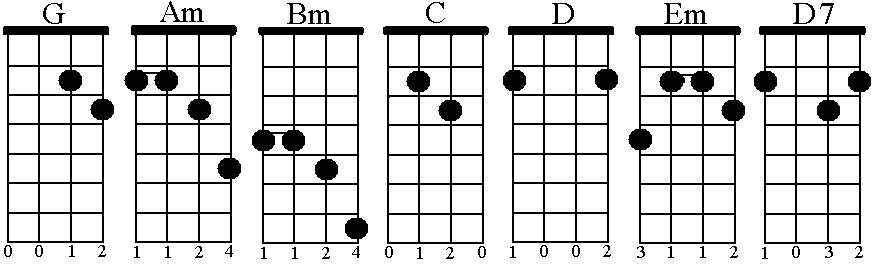
\includegraphics[width = .5\textwidth]{../../../pngs/mand_ch_key_g1}
\end{center}

\begin{guitar}
\begin{multicols}{2}
\textbf{Intro:}
G  G/D  x4
 
\textbf{Verse 1:}
[G]  Almost Heaven,[Em] West Virginia,
[D] Blue Ridge Mountains, [C]Shenandoah [G]River.
Life is old there, [Em]older than the trees,
[D]younger than the mountains,
[C]growin' like a breeze[G].
 
\textbf{Chorus:}
Country [G]Roads, take me [D]home, to the
[Em]place I be[C]long West Vir[G]ginia,
mountain [D]mama, take me [C]home,
country [G]roads.
\textbf{Verse 2:}\\
\textbf{Chorus:}\\
\textbf{Bridge:}
[Em] I hear her [D]voice, in the [G]mornin' hour she calls me.
The [C]radio re[G]minds me of my [D]home far away.
And [Em]drivin' down the [F]road I get a [C]feelin' that I [G]should have been home [D]yesterday, yester[D7]day.
\textbf{Chorus}\\% Maybe x2 

\textbf{Outro}
Take me [D]home, (down) country [G]roads.
Take me [D]home, (down) country [G]roads.
\end{multicols}

\vspace{-3em}
\begin{center}
\textit{Additional lyrics:}
\end{center}

\tiny\flushleft
\vspace{-7em}

\textbf{Verse 2:}
All my memories  gather 'round her,
miner's lady, stranger to blue water.
Dark and dusty, painted on the sky,
misty taste of moonshine,
teardrop in my eye.

\end{guitar}
\end{document}